\documentclass{standalone}
\usepackage{tikz}
\usetikzlibrary{patterns, positioning}


\begin{document}
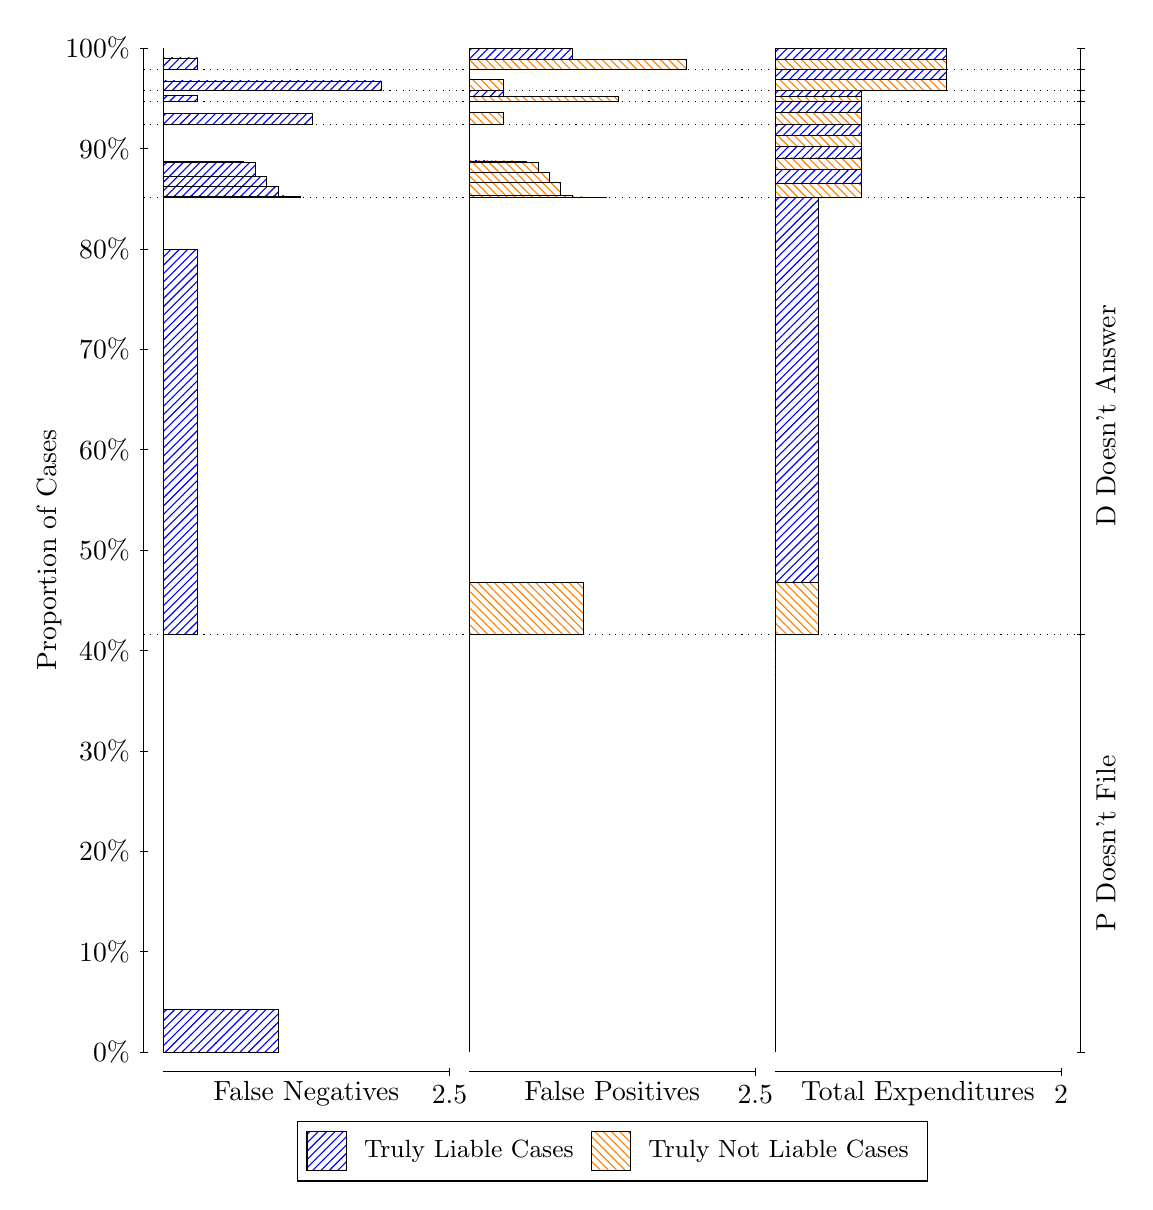
\begin{tikzpicture}
\draw[black, very thin] (1.5,1.75) -- (1.5,14.5);
\node[rotate=90, text=black, anchor=center] at (0.3, 8.125) {Proportion of Cases};
\draw[black, very thin] (1.45,1.75) -- (1.55,1.75);
\node[text=black, anchor=east] at (1.45, 1.75) {0\%};
\draw[black, very thin] (1.45,3.025) -- (1.55,3.025);
\node[text=black, anchor=east] at (1.45, 3.025) {10\%};
\draw[black, very thin] (1.45,4.3) -- (1.55,4.3);
\node[text=black, anchor=east] at (1.45, 4.3) {20\%};
\draw[black, very thin] (1.45,5.575) -- (1.55,5.575);
\node[text=black, anchor=east] at (1.45, 5.575) {30\%};
\draw[black, very thin] (1.45,6.85) -- (1.55,6.85);
\node[text=black, anchor=east] at (1.45, 6.85) {40\%};
\draw[black, very thin] (1.45,8.125) -- (1.55,8.125);
\node[text=black, anchor=east] at (1.45, 8.125) {50\%};
\draw[black, very thin] (1.45,9.4) -- (1.55,9.4);
\node[text=black, anchor=east] at (1.45, 9.4) {60\%};
\draw[black, very thin] (1.45,10.675) -- (1.55,10.675);
\node[text=black, anchor=east] at (1.45, 10.675) {70\%};
\draw[black, very thin] (1.45,11.95) -- (1.55,11.95);
\node[text=black, anchor=east] at (1.45, 11.95) {80\%};
\draw[black, very thin] (1.45,13.225) -- (1.55,13.225);
\node[text=black, anchor=east] at (1.45, 13.225) {90\%};
\draw[black, very thin] (1.45,14.5) -- (1.55,14.5);
\node[text=black, anchor=east] at (1.45, 14.5) {100\%};

\draw[black, very thin] (13.4,1.75) -- (13.4,14.5);
\draw[black, very thin] (13.35,1.75) -- (13.45,1.75);
\node[anchor=west] at (13.35, 1.75) {};
\draw[black, very thin] (13.35,7.0516) -- (13.45,7.0516);
\node[anchor=west] at (13.35, 7.0516) {};
\draw[black, very thin] (13.35,12.605) -- (13.45,12.605);
\node[anchor=west] at (13.35, 12.605) {};
\draw[black, very thin] (13.35,13.527) -- (13.45,13.527);
\node[anchor=west] at (13.35, 13.527) {};
\draw[black, very thin] (13.35,13.824) -- (13.45,13.824);
\node[anchor=west] at (13.35, 13.824) {};
\draw[black, very thin] (13.35,13.959) -- (13.45,13.959);
\node[anchor=west] at (13.35, 13.959) {};
\draw[black, very thin] (13.35,14.227) -- (13.45,14.227);
\node[anchor=west] at (13.35, 14.227) {};
\draw[black, very thin] (13.35,14.5) -- (13.45,14.5);
\node[anchor=west] at (13.35, 14.5) {};

\draw[black, very thin, pattern color=blue, pattern=north east lines] (1.75,1.75) rectangle (3.2033,2.2912);
\draw[black, very thin, pattern color=orange, pattern=north west lines] (1.75,2.2912) rectangle (1.75,7.0516);
\draw[black, very thin, pattern color=blue, pattern=north east lines] (1.75,7.0516) rectangle (2.186,11.94);
\draw[black, very thin, pattern color=orange, pattern=north west lines] (1.75,11.94) rectangle (1.75,12.605);
\draw[black, very thin, pattern color=blue, pattern=north east lines] (1.75,12.605) rectangle (3.494,12.612);
\draw[black, very thin, pattern color=blue, pattern=north east lines] (1.75,12.612) rectangle (3.3487,12.623);
\draw[black, very thin, pattern color=blue, pattern=north east lines] (1.75,12.623) rectangle (3.2033,12.747);
\draw[black, very thin, pattern color=blue, pattern=north east lines] (1.75,12.747) rectangle (3.058,12.749);
\draw[black, very thin, pattern color=blue, pattern=north east lines] (1.75,12.749) rectangle (3.058,12.874);
\draw[black, very thin, pattern color=blue, pattern=north east lines] (1.75,12.874) rectangle (2.9127,13.046);
\draw[black, very thin, pattern color=blue, pattern=north east lines] (1.75,13.046) rectangle (2.7673,13.06);
\draw[black, very thin, pattern color=blue, pattern=north east lines] (1.75,13.06) rectangle (2.622,13.064);
\draw[black, very thin, pattern color=blue, pattern=north east lines] (1.75,13.064) rectangle (2.4767,13.065);
\draw[black, very thin, pattern color=blue, pattern=north east lines] (1.75,13.065) rectangle (2.3313,13.065);
\draw[black, very thin, pattern color=orange, pattern=north west lines] (1.75,13.065) rectangle (1.75,13.527);
\draw[black, very thin, pattern color=blue, pattern=north east lines] (1.75,13.527) rectangle (3.6393,13.669);
\draw[black, very thin, pattern color=orange, pattern=north west lines] (1.75,13.669) rectangle (1.75,13.824);
\draw[black, very thin, pattern color=blue, pattern=north east lines] (1.75,13.824) rectangle (2.186,13.895);
\draw[black, very thin, pattern color=orange, pattern=north west lines] (1.75,13.895) rectangle (1.75,13.959);
\draw[black, very thin, pattern color=blue, pattern=north east lines] (1.75,13.959) rectangle (4.5113,14.083);
\draw[black, very thin, pattern color=orange, pattern=north west lines] (1.75,14.083) rectangle (1.75,14.227);
\draw[black, very thin, pattern color=blue, pattern=north east lines] (1.75,14.227) rectangle (2.186,14.376);
\draw[black, very thin, pattern color=orange, pattern=north west lines] (1.75,14.376) rectangle (1.75,14.5);
\draw[black, very thin, pattern color=orange, pattern=north west lines] (5.6333,1.75) rectangle (5.6333,6.5104);
\draw[black, very thin, pattern color=blue, pattern=north east lines] (5.6333,6.5104) rectangle (5.6333,7.0516);
\draw[black, very thin, pattern color=orange, pattern=north west lines] (5.6333,7.0516) rectangle (7.0867,7.7166);
\draw[black, very thin, pattern color=blue, pattern=north east lines] (5.6333,7.7166) rectangle (5.6333,12.605);
\draw[black, very thin, pattern color=orange, pattern=north west lines] (5.6333,12.605) rectangle (7.3773,12.606);
\draw[black, very thin, pattern color=orange, pattern=north west lines] (5.6333,12.606) rectangle (7.232,12.606);
\draw[black, very thin, pattern color=orange, pattern=north west lines] (5.6333,12.606) rectangle (7.0867,12.61);
\draw[black, very thin, pattern color=orange, pattern=north west lines] (5.6333,12.61) rectangle (6.9413,12.624);
\draw[black, very thin, pattern color=orange, pattern=north west lines] (5.6333,12.624) rectangle (6.796,12.797);
\draw[black, very thin, pattern color=orange, pattern=north west lines] (5.6333,12.797) rectangle (6.6507,12.923);
\draw[black, very thin, pattern color=orange, pattern=north west lines] (5.6333,12.923) rectangle (6.5053,13.047);
\draw[black, very thin, pattern color=orange, pattern=north west lines] (5.6333,13.047) rectangle (6.36,13.059);
\draw[black, very thin, pattern color=orange, pattern=north west lines] (5.6333,13.059) rectangle (6.2147,13.067);
\draw[black, very thin, pattern color=blue, pattern=north east lines] (5.6333,13.067) rectangle (5.924,13.067);
\draw[black, very thin, pattern color=blue, pattern=north east lines] (5.6333,13.067) rectangle (5.7787,13.067);
\draw[black, very thin, pattern color=blue, pattern=north east lines] (5.6333,13.067) rectangle (5.6333,13.527);
\draw[black, very thin, pattern color=orange, pattern=north west lines] (5.6333,13.527) rectangle (6.0693,13.682);
\draw[black, very thin, pattern color=blue, pattern=north east lines] (5.6333,13.682) rectangle (5.6333,13.824);
\draw[black, very thin, pattern color=orange, pattern=north west lines] (5.6333,13.824) rectangle (7.5227,13.888);
\draw[black, very thin, pattern color=blue, pattern=north east lines] (5.6333,13.888) rectangle (6.0693,13.959);
\draw[black, very thin, pattern color=orange, pattern=north west lines] (5.6333,13.959) rectangle (6.0693,14.104);
\draw[black, very thin, pattern color=blue, pattern=north east lines] (5.6333,14.104) rectangle (5.6333,14.227);
\draw[black, very thin, pattern color=orange, pattern=north west lines] (5.6333,14.227) rectangle (8.3947,14.352);
\draw[black, very thin, pattern color=blue, pattern=north east lines] (5.6333,14.352) rectangle (6.9413,14.5);
\draw[black, very thin, pattern color=orange, pattern=north west lines] (9.5167,1.75) rectangle (9.5167,6.5104);
\draw[black, very thin, pattern color=blue, pattern=north east lines] (9.5167,6.5104) rectangle (9.5167,7.0516);
\draw[black, very thin, pattern color=orange, pattern=north west lines] (9.5167,7.0516) rectangle (10.062,7.7166);
\draw[black, very thin, pattern color=blue, pattern=north east lines] (9.5167,7.7166) rectangle (10.062,12.605);
\draw[black, very thin, pattern color=orange, pattern=north west lines] (9.5167,12.605) rectangle (10.607,12.782);
\draw[black, very thin, pattern color=blue, pattern=north east lines] (9.5167,12.782) rectangle (10.607,12.959);
\draw[black, very thin, pattern color=orange, pattern=north west lines] (9.5167,12.959) rectangle (10.607,13.104);
\draw[black, very thin, pattern color=blue, pattern=north east lines] (9.5167,13.104) rectangle (10.607,13.247);
\draw[black, very thin, pattern color=orange, pattern=north west lines] (9.5167,13.247) rectangle (10.607,13.387);
\draw[black, very thin, pattern color=blue, pattern=north east lines] (9.5167,13.387) rectangle (10.607,13.527);
\draw[black, very thin, pattern color=orange, pattern=north west lines] (9.5167,13.527) rectangle (10.607,13.682);
\draw[black, very thin, pattern color=blue, pattern=north east lines] (9.5167,13.682) rectangle (10.607,13.824);
\draw[black, very thin, pattern color=orange, pattern=north west lines] (9.5167,13.824) rectangle (10.607,13.888);
\draw[black, very thin, pattern color=blue, pattern=north east lines] (9.5167,13.888) rectangle (10.607,13.959);
\draw[black, very thin, pattern color=orange, pattern=north west lines] (9.5167,13.959) rectangle (11.697,14.104);
\draw[black, very thin, pattern color=blue, pattern=north east lines] (9.5167,14.104) rectangle (11.697,14.227);
\draw[black, very thin, pattern color=orange, pattern=north west lines] (9.5167,14.227) rectangle (11.697,14.352);
\draw[black, very thin, pattern color=blue, pattern=north east lines] (9.5167,14.352) rectangle (11.697,14.5);
\draw[black, dotted] (1.5,7.0516) -- (13.4,7.0516);
\draw[black, dotted] (1.5,12.605) -- (13.4,12.605);
\draw[black, dotted] (1.5,13.527) -- (13.4,13.527);
\draw[black, dotted] (1.5,13.824) -- (13.4,13.824);
\draw[black, dotted] (1.5,13.959) -- (13.4,13.959);
\draw[black, dotted] (1.5,14.227) -- (13.4,14.227);
\draw[black, very thin] (1.75,1.5) -- (5.3833,1.5);
\node[text=black, anchor=north] at (3.5667, 1.5) {False Negatives};
\draw[black, very thin] (5.3833,1.45) -- (5.3833,1.55);
\node[text=black, anchor=north] at (5.3833, 1.45) {2.5};

\draw[black, very thin] (5.6333,1.5) -- (9.2667,1.5);
\node[text=black, anchor=north] at (7.45, 1.5) {False Positives};
\draw[black, very thin] (9.2667,1.45) -- (9.2667,1.55);
\node[text=black, anchor=north] at (9.2667, 1.45) {2.5};

\draw[black, very thin] (9.5167,1.5) -- (13.15,1.5);
\node[text=black, anchor=north] at (11.333, 1.5) {Total Expenditures};
\draw[black, very thin] (13.15,1.45) -- (13.15,1.55);
\node[text=black, anchor=north] at (13.15, 1.45) {2};

\node[text=black, centered, rotate=90] at (13.72, 4.4008) {P Doesn't File};
\node[text=black, centered, rotate=90] at (13.72, 9.8284) {D Doesn't Answer};






\draw (7.449999999999999,1.5) node[draw=none] (baseCoordinate) {};
\begin{scope}[align=center]
        \matrix[scale=0.5, draw=black, below=0.5cm of baseCoordinate, nodes={draw}, column sep=0.1cm]{
            \node[rectangle, draw, minimum width=0.5cm, minimum height=0.5cm, pattern color=blue, pattern=north east lines] {}; &
            \node[draw=none, font=\small, text=black] (B) {Truly Liable Cases}; &
            \node[rectangle, draw, minimum width=0.5cm, minimum height=0.5cm, pattern color=orange, pattern=north west lines] {}; &
            \node[draw=none, font=\small, text=black] (B) {Truly Not Liable Cases}; \\
            };
\end{scope}

\end{tikzpicture}
\end{document}